\documentclass{urticle}

\begin{document}

\begin{center}
{\LARGE \textbf{Исследование коннектом и когнетом}}

{\Large Мокров Никита}

{\large Московский Физико-Технический Институт}

{\large Факультет Радиотехники и Кибернетики}

{\large mokrov@frtk.ru}
\end{center}

\section*{Введение}
\subsection*{Постановка задачи}
Термин «коннектом» предложен в 2005 году независимо двумя исследователями Олафом Спорнсом и Патриком Хэгмэнном по аналогии с «геномом» (полное описание всех генов) и «протеомом» (полное описание строения и функций всех белков). Сегодня под «коннектомом» понимают полное описание связей в нервной системе того или иного организма.

Как известно, главной задачей нейронаук является понимание того, как из работы материальных и доступных изучению приборами элементов нервной системы получается неуловимая работа психики. Создание сетевых моделей формальных элементов мозга (когнитома) — всего лишь один из этапов. Наш соотечественник Константин Анохин вводит новый термин «ког» — элемент психического опыта, связанный с работой какого-то участка нейронной сети. Из множества связанных друг с другом когов строится когнитом — сеть психики, внутренний мир животного или человека, которому принадлежит данная нейронная сеть.

С точки зрения математики, мы можем представить человеческий мозг в виде взвешенного графа взаимодействия отдельных его участков. Этот факт дает широкие возможности для большого спектра задач. Одна из таких - задача машинного обучения: как по коннектому и когнетому определить ту или иную болезнь человека на ранней стадии.

\subsection*{Методы решения и подходы}
На данный момент эта задача решается широким кругом лиц из всех стран мира. Ислледования ведутся в различных напрвлениях: применяются как классические метода машинного обучения, так и используютя новые методы. В данном отчете исследование основывается на работе по повышению классификации путем сочетания различных нормировок\cite{article1}. 

В данной работе приведены следующие методы нормализации:
\begin{itemize}
	\item Оригинальная нормализация
	\item Бинарная нормализация
	\item Геометрическая нормализация
	\item Топологическая нормализация			
\end{itemize}

С помощью данного подходы, можно учесть многие харакетристики графа. Основываясь на данном методе были получены существенные результаты\cite{article1} для области машинного обучения в нейронауках.

\section*{Альтернативный подход}
В данной статье использовались данные людей здоровых и больных аутизмом (UCLA Multimodal Connectivity Database), которые содержат порядка 100 матриц смежности размера (264, 264) для графов, которые и представляют когнетом пациента.

Из-за этого мы сталкиваемся с проблемой большого количества входных признаков. В этой работе была проверена теория\footnote{Данная теория пренадлежит Максиму Панову} о том, что исходные данные сильно зашумлены. Во-первых, это следует из того, что каждая нервная клетка обновляет силу связи между смежными нейронными, и поэтому мы строим модель для опрделенного момента времени и состояния человека. Во-вторых, обработка данных проводилось вручную, путем сравнения послойных участков.

Для решения этой проблемы, воспользуемся спектральным разложением (Или что тоже самое для симметричной матрицы - сингулярное разложение). 
$$ A = V \Lambda {V}^{-1} $$
После чего, будет использовать вместо матрицы $A$, матрицу $A'$
$$ A' = V \Lambda $$
Теперь, вместо того, чтобы использовать все собственные вектора и значения, возмем только $k$ самых больших собственных значений и векторов, соответсвующие им. Таким образом, вместо матрицы размером $(N, N)$, мы будем использовать матрицу размера $(N, N-k)$.

\section*{Результаты}
Обучив логистиечскую регрессию на новой матрице для 100 раличных валидаций, мы получим завсимость значения по метрике Roc Auc от параметра $k$, который указывает на количество выкинутых собственных значений и собственных векторов.

\begin{figure}[H]
	\centering{
	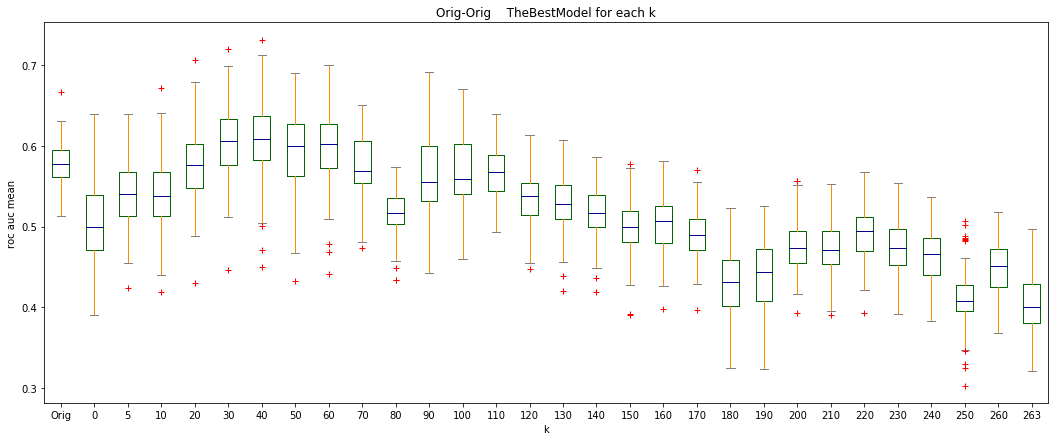
\includegraphics[width=160mm]{1.png}
	}
	\caption{Boxplot для оригинальной матрицы в зависимости от $k$}
	\label{f1}
\end{figure}

Чаще всего получается так, что лучшее решение является объединением двух или более других методов. Перед тем как понижать размерность матрицы $A$, можно по-разному ee нормализовать.
Если вопспользоваться бинарной нормировкой, то результат смотрится гараздо лучше и видна более четкая зависимость.
\begin{figure}[H]
	\noindent\centering{
	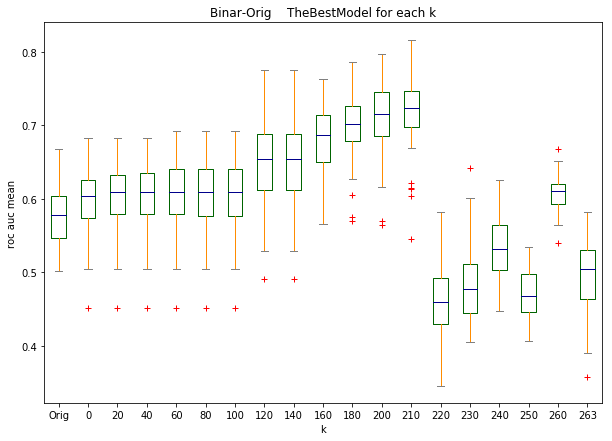
\includegraphics[width=120mm]{2.png}
	}
	\caption{Boxplot для бинарной матрицы в зависимости от $k$}
	\label{f}
\end{figure}

Данный метод был опробован на дргуих данныx (APOE-4), которые содержат пары (матрица размером (68, 68) и метка класса). Проведем тот же алогритм на бинарной нормировке и получим такие значения для 100 различных валидаций.

\begin{figure}[H]
	\noindent\centering{
	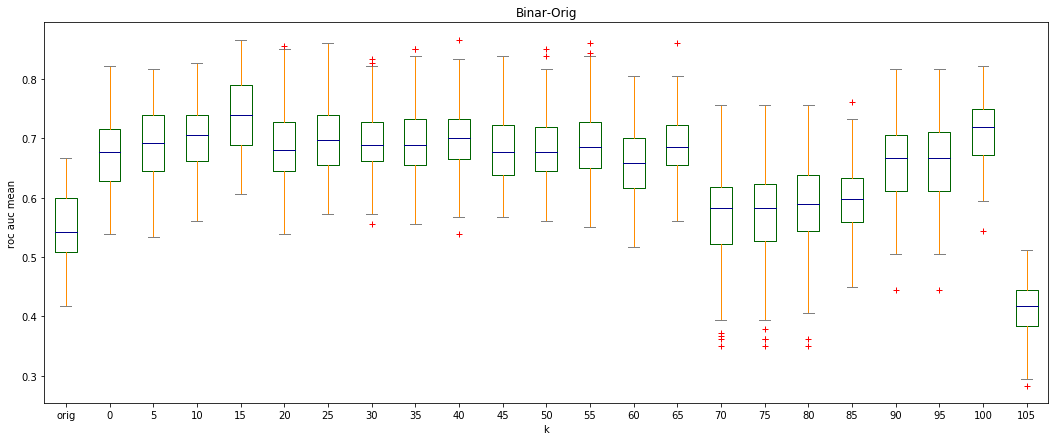
\includegraphics[width=160mm]{3.png}
	}
	\caption{Boxplot для бинарной матрицы в зависимости от $k$}
	\label{f3}
\end{figure}

Стоит отметить, что как в работе\cite{article1}, так в работе\cite{article2}, в которой применялся подход ядра, бинарная нормировка не давала приемущества перед другими. Напротив, в данном исследовании, такой тип предобработки данных был более удачен. С помощью этого метода удалось увеличить результат для обоих данных, в сравнении с использованием оригинаьной матрицы, как целевой переменной.

\begin{center}
\begin{tabular}[t]{|c|c|c|}
\hline
	Данные & Результат для $A$ & Результат для $A'$ \\
\hline
	UCLAbaseline & 0.58 & 0.72 \\
\hline
	APOE-4 & 0.54 & 0.73 \\
\hline
\end{tabular}
\end{center}

\section*{Заключение}
Как можно заметить, используя только более информативные признаки матрицы (собственные вектора, умноженные на собственные значения), результат может улучишься для правильной первоначальной нормировки данных.

Возникает вопрос, почему при использовании оригинальной матрицы результат существенно отличается, если использовать матрицу с бинарной нормировкой? Другими словами, нам не так важно, как сильно взаимодействую два конкретных участка мозга. А важно нам только наличие или отсуствие этой связи.

При более обширных исследованиях, возникают новые вопросы такого рода, на которых нет четских ответов и правильных рассуждений.

\begin{thebibliography}{2}
\bibitem{article1} Boosting Connectome Classification via Combination of Geometric and Topological Normalizations by Dmitry Petrov, Yulia Dodonova, Leonid Zhukov and Mikhail Belyaev
\bibitem{article2} Machine Learning Application to Human Brain Network Studies: A Kernel Approach by Anvar Kurmukov, Yulia Dodonova and Leonid Zhukov 
\end{thebibliography}

\end{document}
